\section{Preliminary questions and EDA}
\begin{itemize}
    \item Which department made the highest turnover in 2016?\par \textbf{Answer:} Department with the highest turnover in year 2016 is, 127.

    \item What are the top 5-week numbers (1 to 53) for department 88 in 2015 in terms of turnover over all stores?\par \textbf{Answer:} Table \ref{tab:top5weeks}
    \begin{table}[htbp]
        \centering
        \caption{Top 5 Performing Weeks}
        \label{tab:top5weeks}
        \begin{tabular}{|c|c|c|c|}
          \hline
          \textbf{Week} & \textbf{Business Unit ID} & \textbf{Department Number} & \textbf{Turnover} \\
          \hline
          2015-01-10 & 132 & 88 & 2306.643525 \\
          2015-07-11 & 4 & 88 & 2073.152091 \\
          2015-07-25 & 4 & 88 & 2070.041381 \\
          2015-07-04 & 4 & 88 & 2028.924124 \\
          2015-09-12 & 11 & 88 & 1935.623844 \\
          \hline
        \end{tabular}
    \end{table}

    \item What was the top performer store in 2014?\par \textbf{Answer:} Table \ref{tab:Top performer store in 2014}
    \begin{table}[h]
        \centering
        \begin{tabular}{|c|c|}
            \hline
            \textbf{Comment} & \textbf{Value} \\
            \hline
            Maximum turnover: & 166858.495\\
            Department with maximum turnover: & 127 \\
            Business unit with maximum turnover: & 121 \\
            \hline
        \end{tabular}
        \caption{Top performer store in 2014.}
        \label{tab:Top performer store in 2014}
    \end{table}   

    \item Based on sales can you guess what kind of sport represents department 73?\par \textbf{Answer:} Figure \ref{fig:1}\par
    Looks like the summer sales, I guess sportswear like swimming, trekking and some shoes and cloths. \par
    In the following figure (deparment-73 and business-18), we can see the average sales were highest during summer and before fall. 
    \begin{figure}[htbp]
        \centering
        \begin{subfigure}[b]{0.45\textwidth}
            \centering
            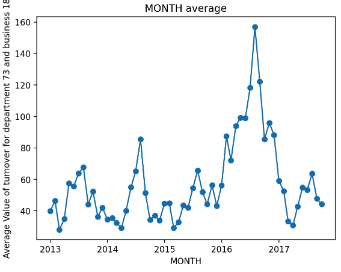
\includegraphics[width=\textwidth]{figures/month_avg_73.png}
            \caption{Monthly average of department 73 business 18}
            \label{fig:1.1}
        \end{subfigure}
        \hfill
        \begin{subfigure}[b]{0.45\textwidth}
            \centering
            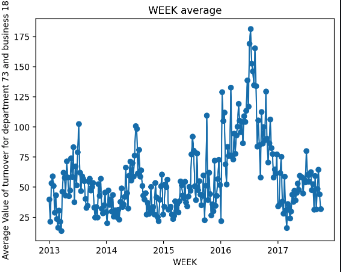
\includegraphics[width=\textwidth]{figures/week_avg_73.png}
            \caption{Monthly average of department 73 business 18}
            \label{fig:1.2}
        \end{subfigure}
        \caption{Average turnover for department 73 business 18}
        \label{fig:1}
    \end{figure}

    \item Based on sales can you guess what kind of sport represents department 117?\par \textbf{Answer:} Figure \ref{fig:2} \par
    Looks like winter sales, I guess it should be related to ski, winter sports, Jackets, wool socks, Shoes, Skies and so on ..\par

    \begin{figure}[htbp]
        \centering
        \begin{subfigure}[b]{0.45\textwidth}
            \centering
            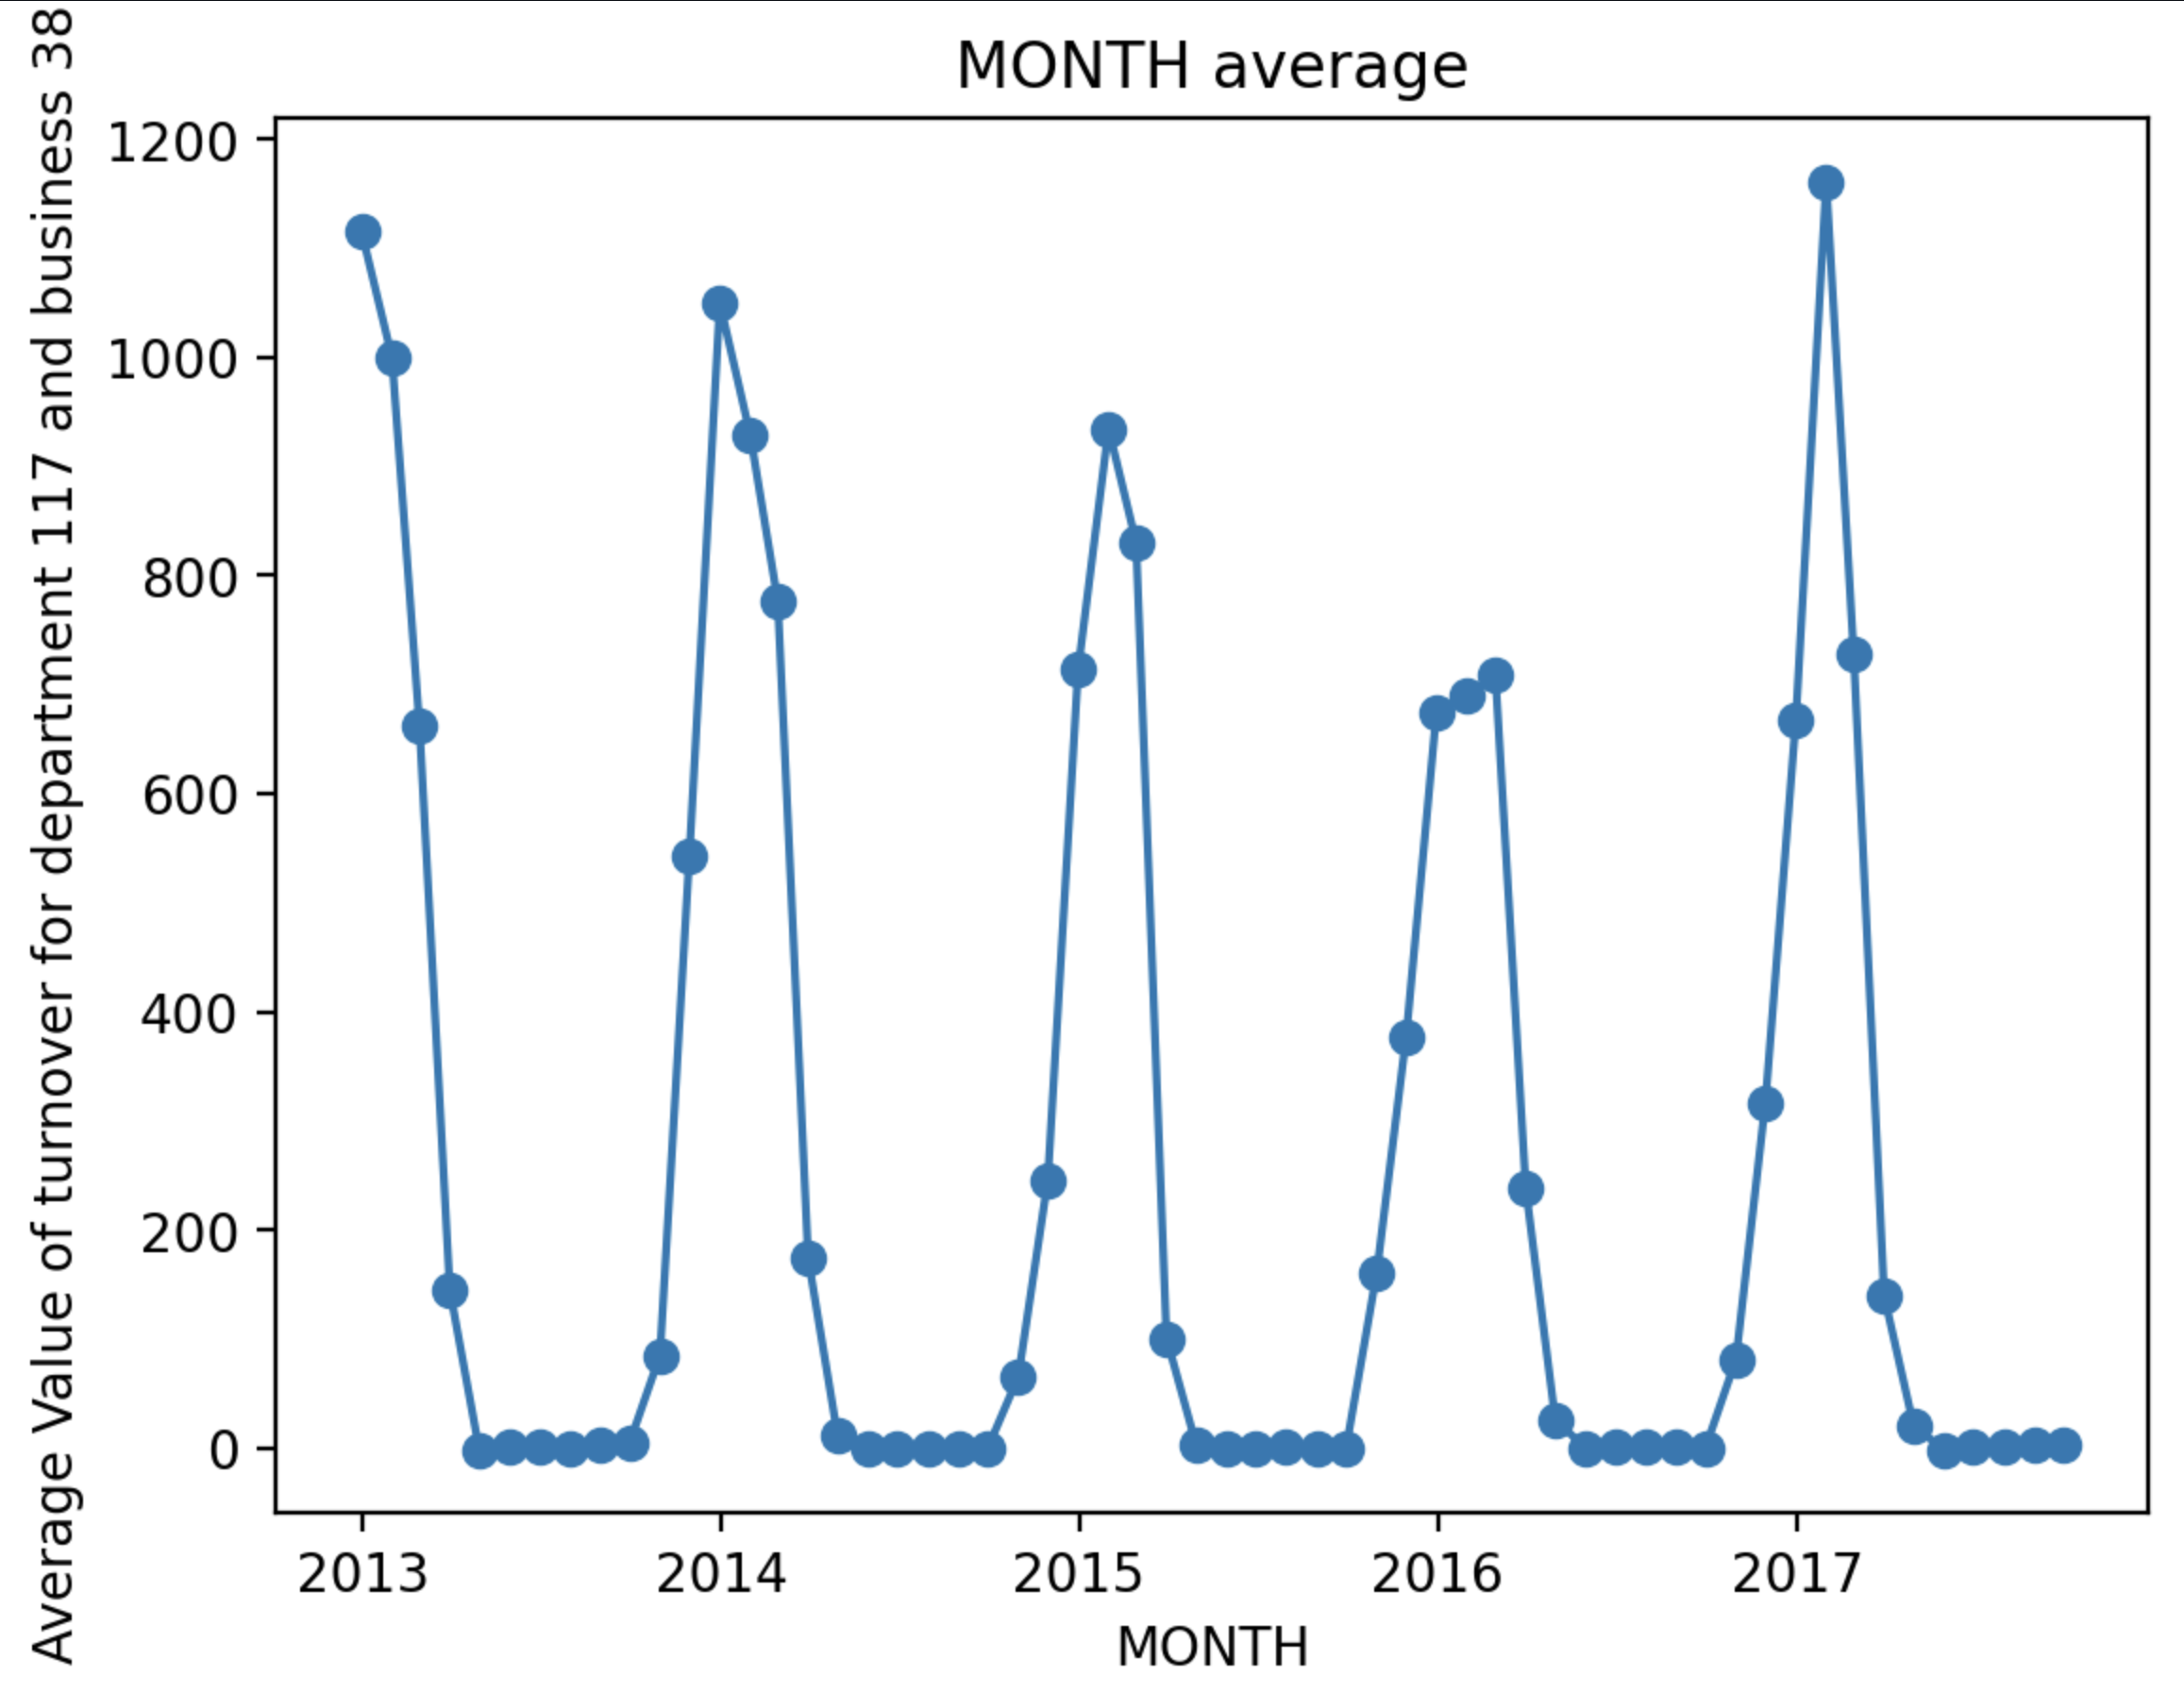
\includegraphics[width=\textwidth]{figures/monthly_avg_117.png}
            \caption{Monthly average of department 117 business 318}
            \label{fig:2.1}
        \end{subfigure}
        \hfill
        \begin{subfigure}[b]{0.45\textwidth}
            \centering
            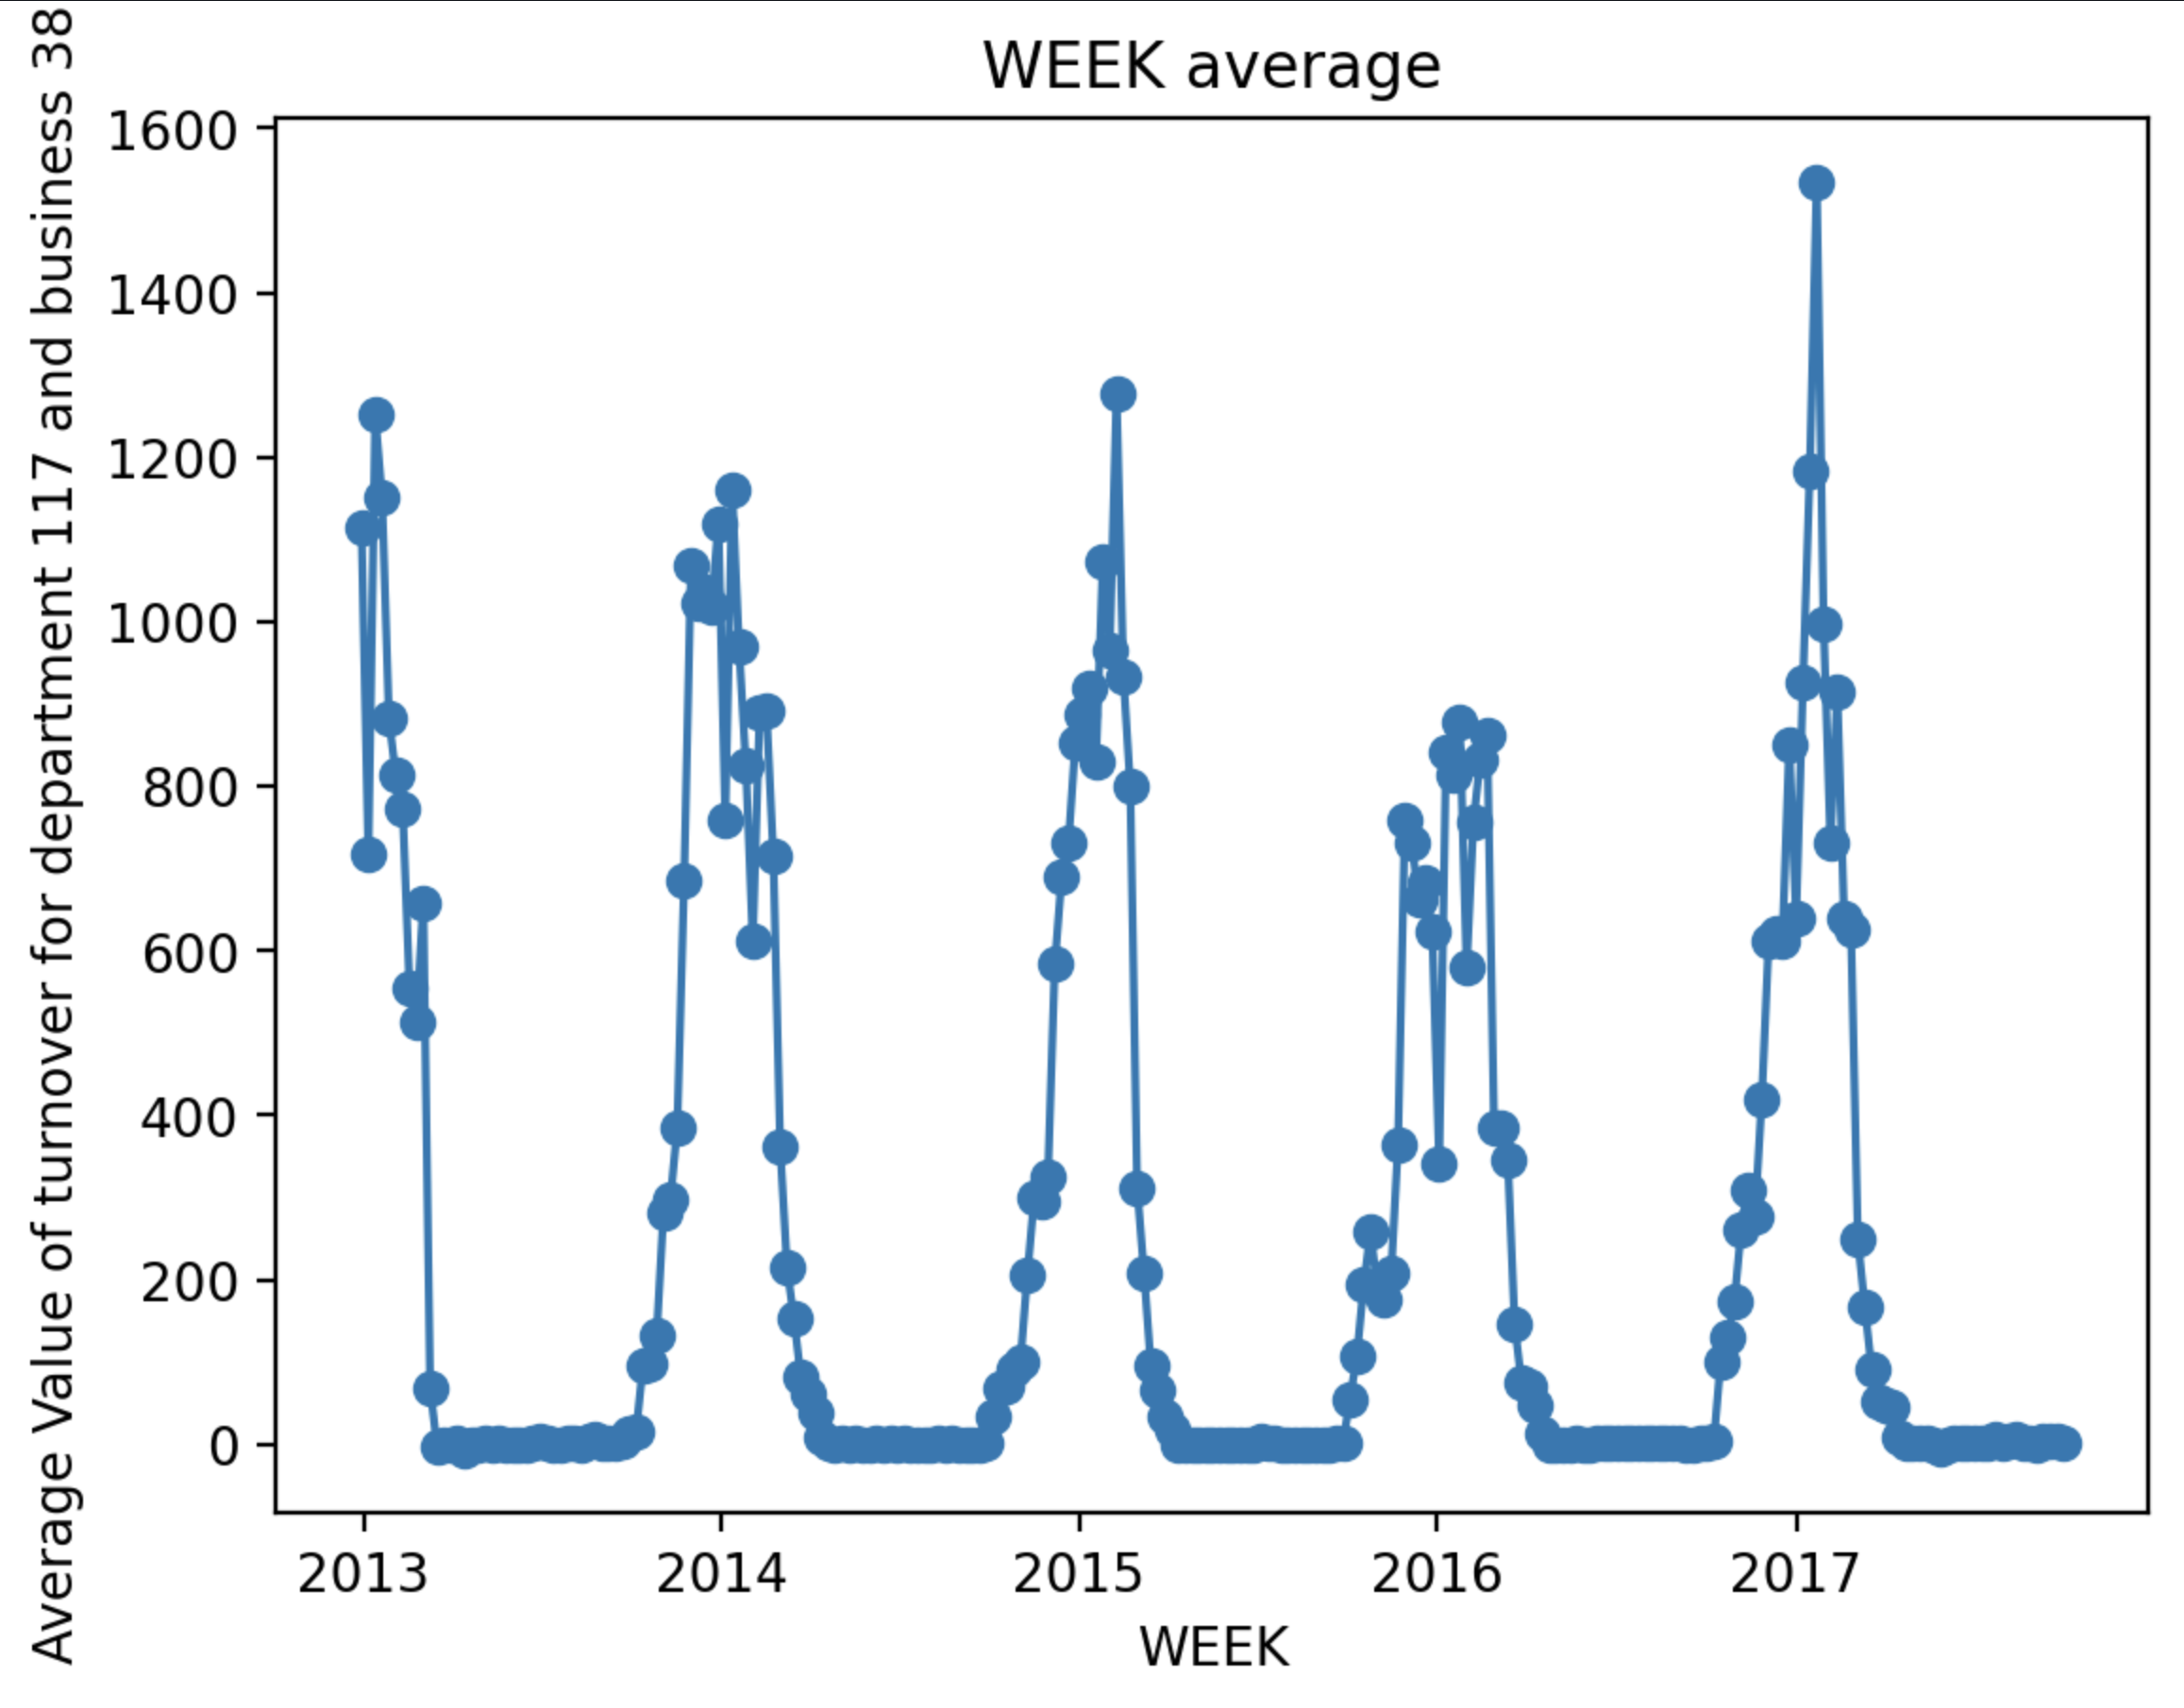
\includegraphics[width=\textwidth]{figures/weekly_avg_117.png}
            \caption{Monthly average of department 117 business 318}
            \label{fig:2.2}
        \end{subfigure}
        \caption{Average turnover for department 117 business 318}
        \label{fig:2}
    \end{figure}

    \item Are the time series stationary? Is this a problem?\par \textbf{Answer:}
    Time series data for certain stores/business units is stationary and others are not. To judge this I looked at the de-trended data, and also we conducted a Dickey-Fuller test. \par
    Stationary time series are easier in prediction when compared to non-stationary time series.
    \item Can the time series be decomposed into several key components?\par \textbf{Answer:}
    Yes, time series can be decomposed into trends, seasonal and residual components. \par
    You can find a code that will help to visualize the trends for a sample data. 

\end{itemize}